\section{Vision}\label{sec: vision}

\begin{wrapfigure}{r} {0.4\linewidth}
    \centering
    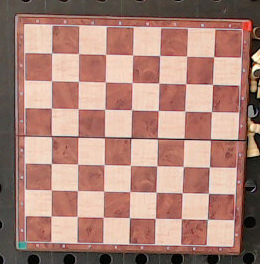
\includegraphics[width=\linewidth]{Pictures/Chessboard with marked corners.png}
    \caption{Image of the chessboard with two corners marked with red and green tape}
    \label{fig: Chessboard with marked corners}
\end{wrapfigure}

As mentioned earlier, the camera needs to find the position of the board and the chess piece moved by the player.
A camera is therefore used to capture an image of the chessboard, which can be processed. Pictures can be seen as 2-dimensional arrays, where each pixel position corresponds to a row and a column, and each position has a value. For example, an RGB picture is therefore 3 2-dimensional arrays, with each matrix corresponding to the 3 different channels (Red, Green, Blue).



The camera identifies the position of the chessboard by detecting pieces of coloured tape placed in two opposite corners. These markers allow for the calculation of a transformation matrix between the robot’s base frame and the board’s frame, and allows the camera to cut down the image to only include the chessboard. An image of the chessboard with the marked corners is shown in \cref{fig: Chessboard with marked corners}.



For this project, HSV (Hue Saturation Value) is used to combat the shadows or changing light on the chessboard, since a change in brightness in theory only affects the value channel. When using HSV, and the colours are black/white, the hue and saturation can be anything and the colour will be registered as the same. To combat this issue a chessboard with texture is used.

\subsection{OpenCV}
The open-source vision library openCV, offers an interface for the camera as well as handling data storage for image processing. \cite{openCV}

\subsection{Placement of the camera}
The placement of the camera determines the perspective distortion of the image. By placing it perpendicular to the table and as far away as possible, the distortion is reduced. This makes it possible to linearly approximate between the coordinates of the pixels, and the real world position.

By placing the camera far away from the chessboard, the picture is bound to include a sizeable amount of noise from the surroundings, as seen on \cref{fig: Raw footage}. As the coloured corners of the chessboard can be difficult to locate in the noisy environment, two larger coloured pegs are placed in opposite corners of the playing space, making them easier to locate. As said in \cref{sec: Workbench setup} these pegs have a known static position, both from the camera and the robot, and are therefore used to define the transformation matrix between the robot's frame and the chessboard. 

\begin{figure} [H]
    \centering
    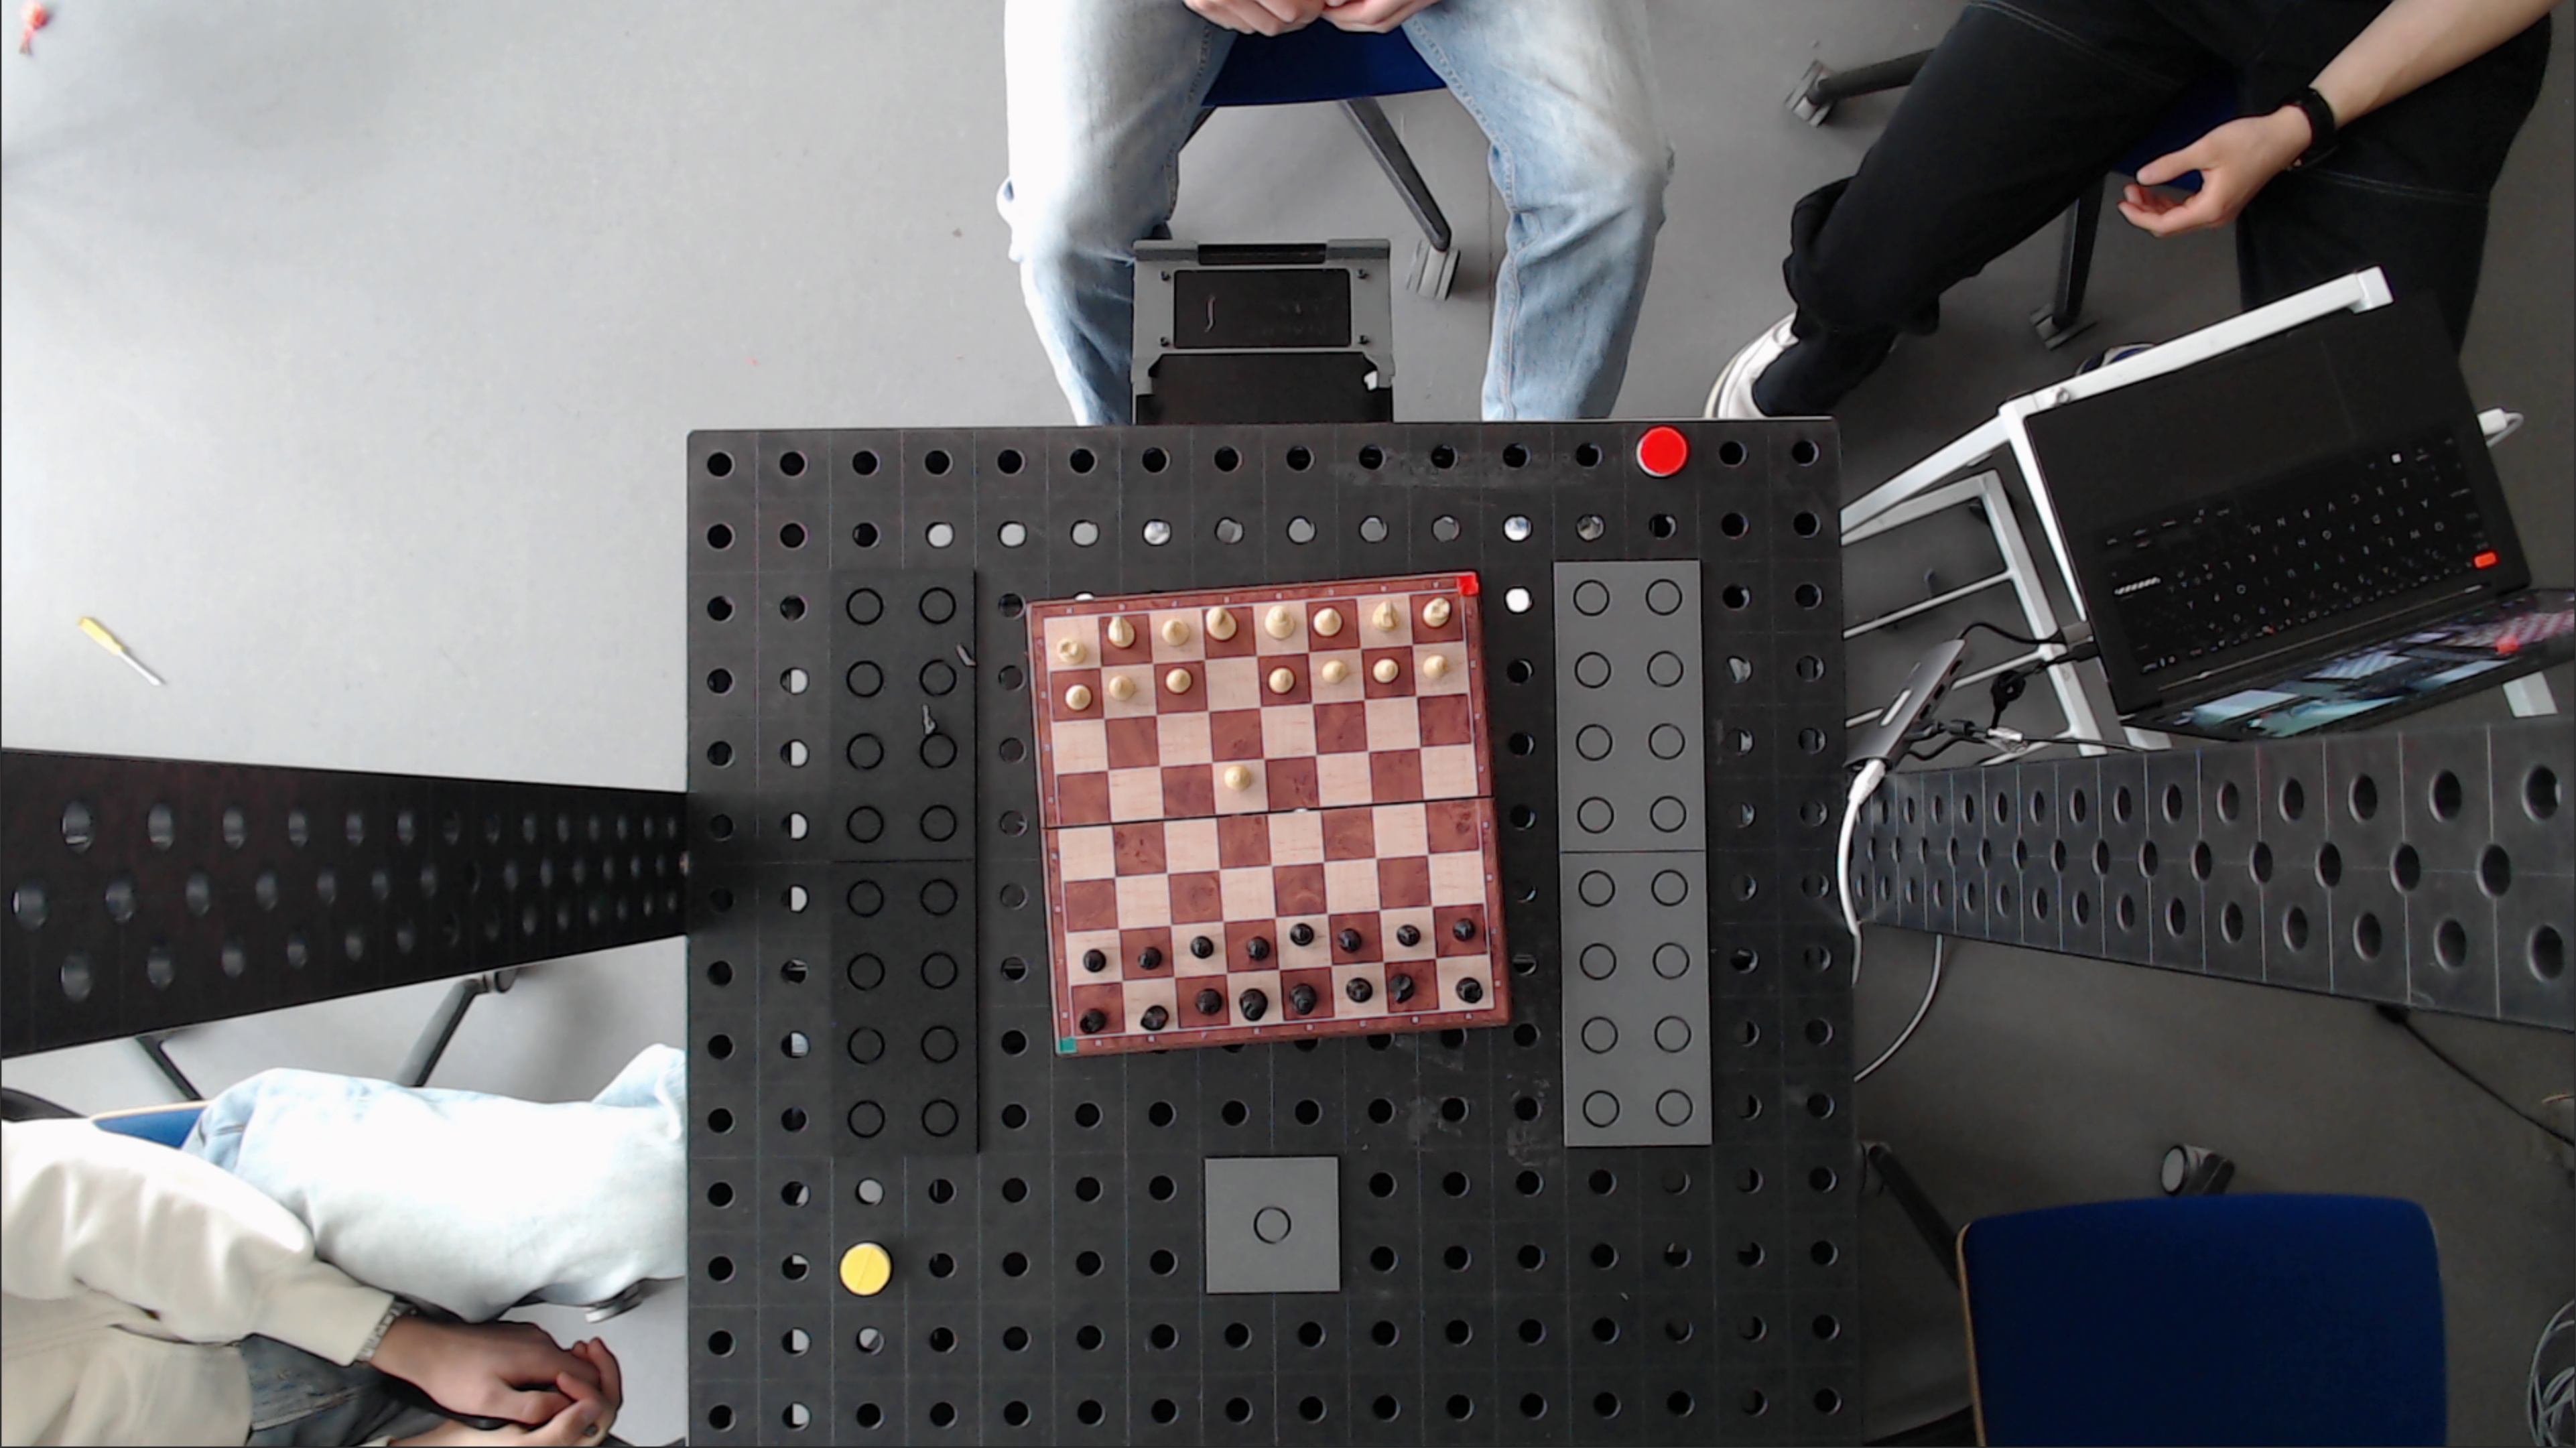
\includegraphics[width=0.6\linewidth]{Pictures/Vision/OriginalImage.png}
    \caption{Camera view}
    \label{fig: Raw footage}
\end{figure}
    

\subsection{Locating different coloured tape} \label{sec: Locate tape}
When looking for the corners and pegs, a specific colour that corresponds to the colour of the tape is used to find where the tape is in the picture. The raw footage is separated into the 3 channels whereafter the colour is subtracted. An example can be seen in \cref{fig:HSVchannels}, where the colour looked for is HSV(179, 100, 85), which corresponds to a green-blueish colour. With the 3 channels separated, a weighted average can be taken to make a singular 1 channel image representing the likelihood of the tape's location. This can be seen in \cref{fig:weightedAverageGreenBoard}

\begin{figure}[H]
    \centering
    \begin{subfigure}[t]{0.19\linewidth}
        \centering
        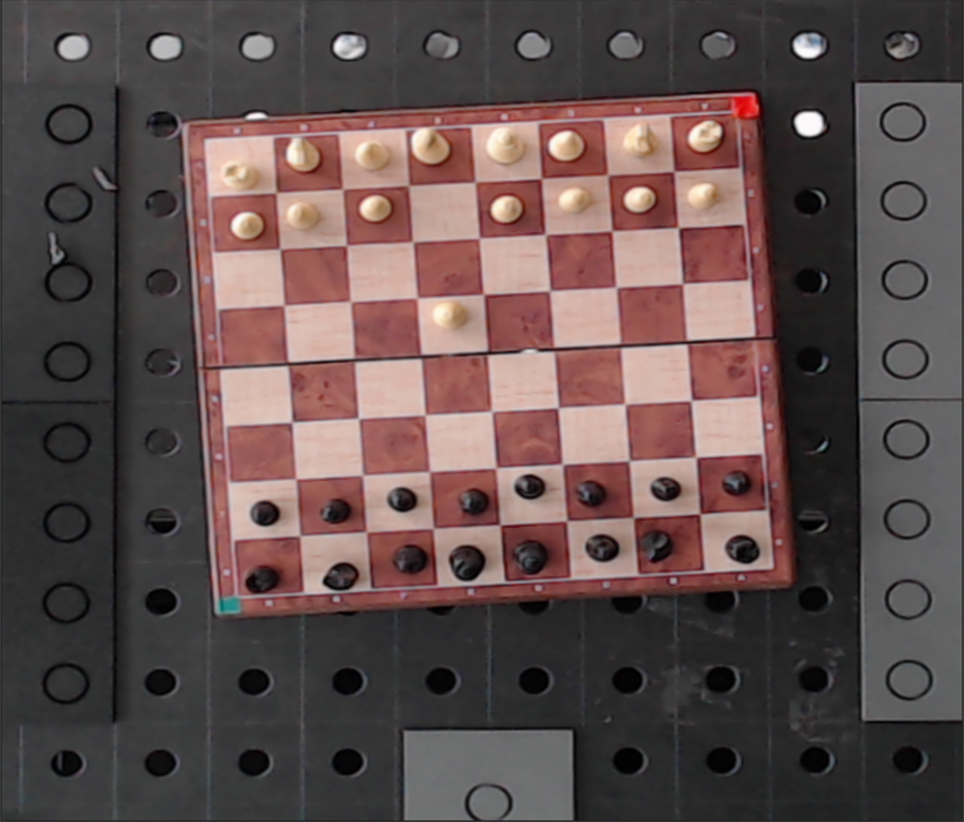
\includegraphics[width=\linewidth]{Pictures/Vision/FirstCut.png}
        \caption{Original image}
        \label{fig:FirstCutGreenBoard}
    \end{subfigure}
    \hfill
    \begin{subfigure}[t]{0.19\linewidth}
        \centering
        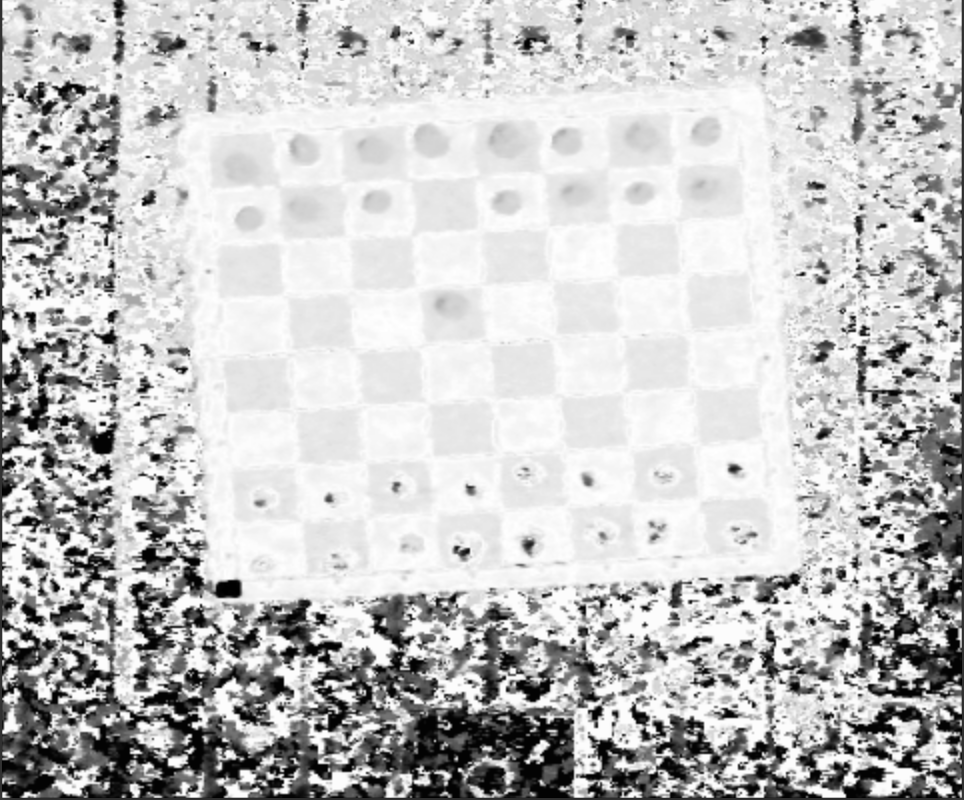
\includegraphics[width=\linewidth]{Pictures/Vision/HueDifferenceGreenBoard.png}
        \caption{Hue difference}
        \label{fig:hueDifferenceGreenBoard}
    \end{subfigure}
    \hfill
    \begin{subfigure}[t]{0.19\linewidth}
        \centering
        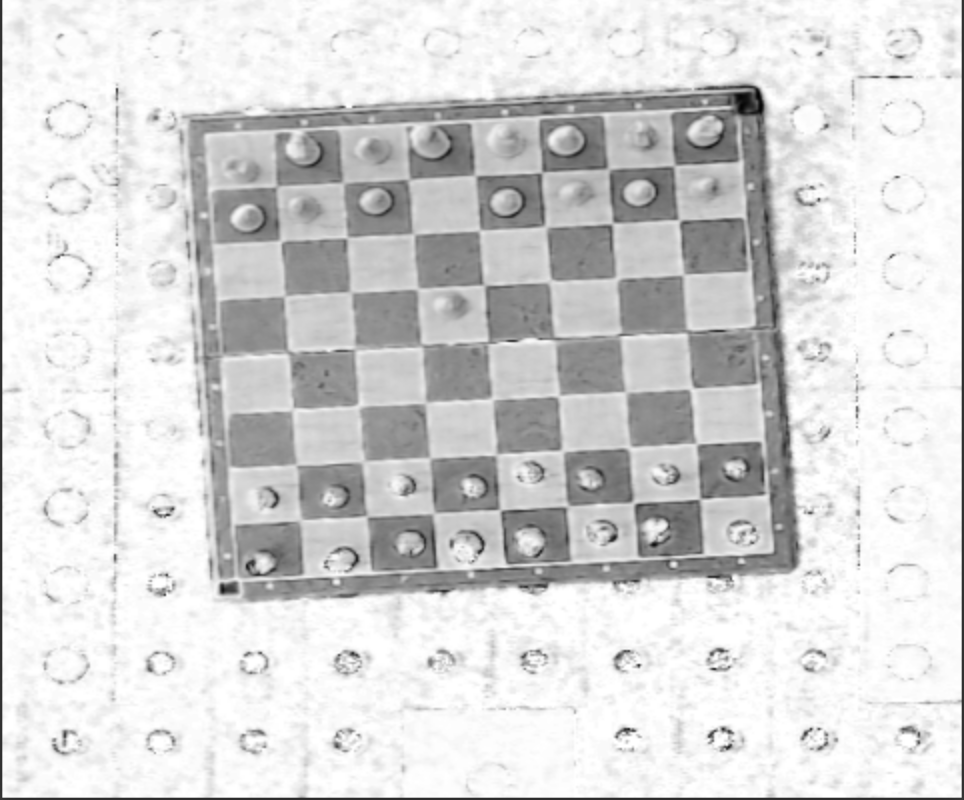
\includegraphics[width=\linewidth]{Pictures/Vision/SaturationDifferenceGreenBoard.png}
        \caption{Saturation difference}
        \label{fig:saturationDiffernceGreenBoard}
    \end{subfigure}
    \hfill
    \begin{subfigure}[t]{0.19\linewidth}
        \centering
        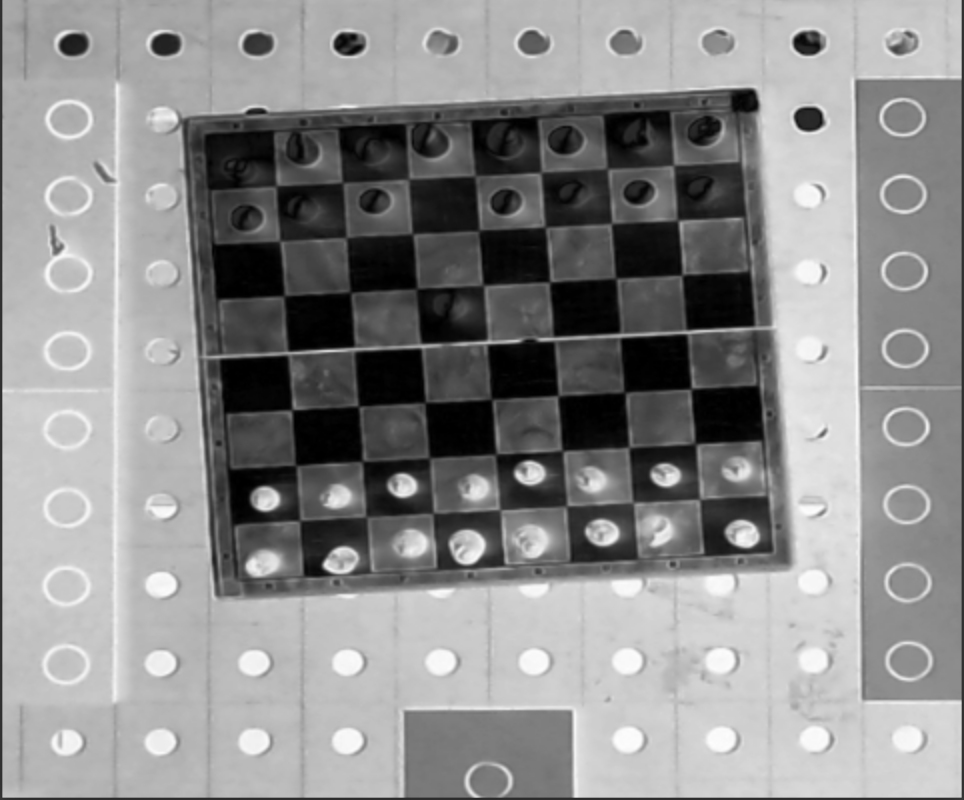
\includegraphics[width=\linewidth]{Pictures/Vision/ValueDifferenceGreenBoard.png}
        \caption{Value difference}
        \label{fig:vlueDiffGreenBoard}
    \end{subfigure}
    \hfill
    \begin{subfigure}[t]{0.19\linewidth}
        \centering
        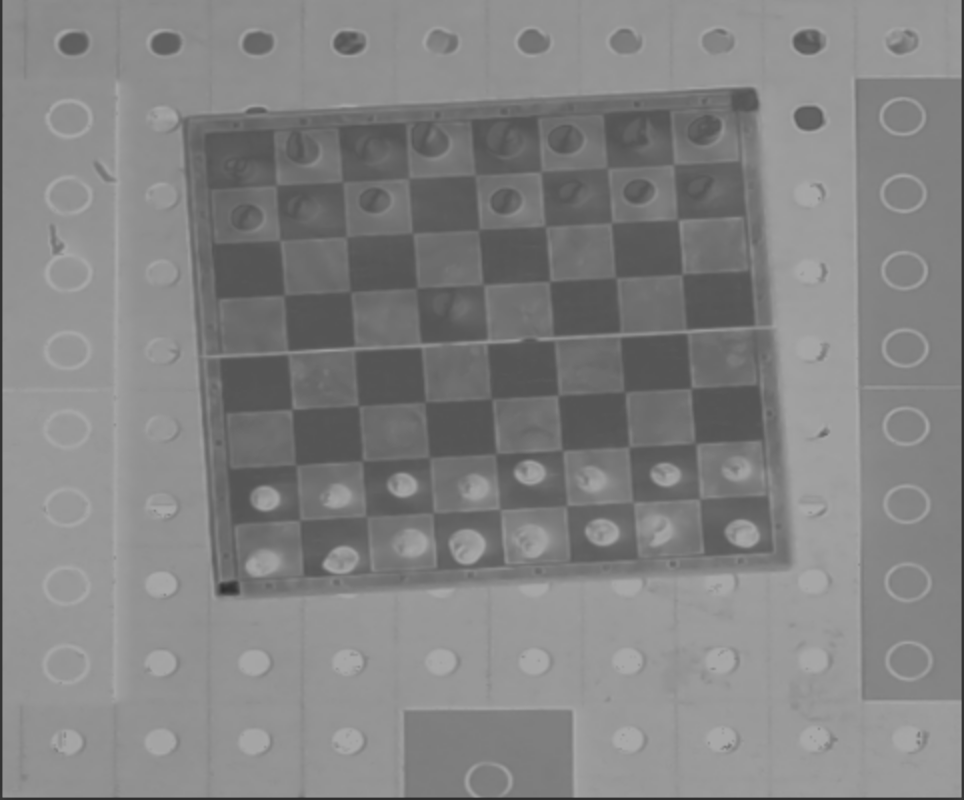
\includegraphics[width=\linewidth]{Pictures/Vision/SummedHSVGreen.png}
        \caption{Weighted average}
        \label{fig:weightedAverageGreenBoard}
    \end{subfigure}
    
    \caption{Original image and its channels difference from the HSV colour HSV(179, 100, 85) and the weighed average. The black spots are the colours most similar to the colour}
    \label{fig:HSVchannels}
\end{figure}

The weight for the channels has been found experimentally, and by looking at the images, after a failed try, to determine which channel is responsible for the fail. The found weight for the 3 channels are: 1 for saturation and value and 2 for the hue channel.

The location of the tape can be determined by finding the area with the lowest values, which corresponds to the black spot in \cref{fig:weightedAverageGreenBoard}.

To make sure we look for a cluster of black spots, and not just a single pixel, a new image can be calculated with \cref{math}
\begin{equation}
    R(x, y)= \sum_{x', y'}(T(x', y') \cdot I(x+x', y+y') \cdot M(x', y')^2
    \label{math}
\end{equation}

Here $R(x, y)$ is the output picture of the result, x and y are the pixel positions in the supplied image, x' and y' are the pixel positions in the template image and $M(x', y')$ is the value of the mask, at the same pixel. The function therefore sums up the product of each pixel on the image and the template. The size of the template image should correspond to the size of the black spot. 
The template being used can be seen in \cref{fig:mask}. The only values close to 0 in the result image is therefore the positions where the black spots in the supplied image are surrounded by other black spots.
OpenCV offers a function to do this called matchTemplate() \cite{openCV}
The result of using this can be seen in \cref{fig:resultOfMatchTemplate()}
\begin{figure}[H]
    \centering
    \begin{subfigure}[t]{0.32\linewidth}
        \centering
        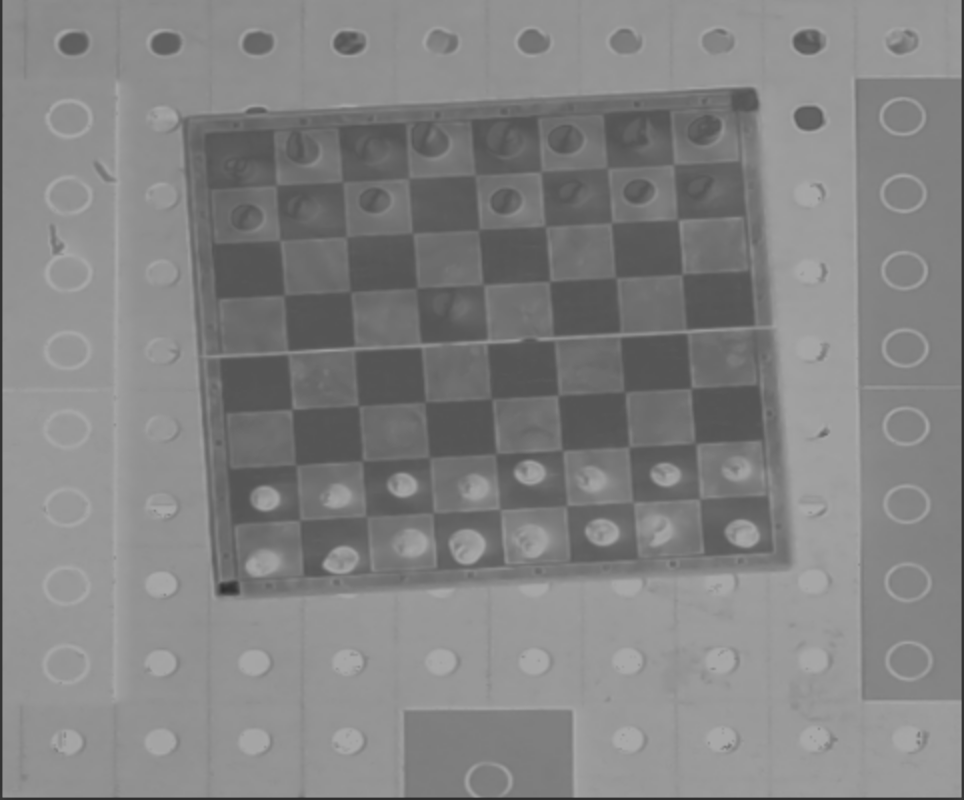
\includegraphics[width=\linewidth]{Pictures/Vision/SummedHSVGreen.png}
        \caption{Weighted average of the different channels}
        \label{fig:weightedAvergeofDiffernetChannels} 
    \end{subfigure}
    \hfill
    \begin{subfigure}[t]{0.32\linewidth}
        \centering
        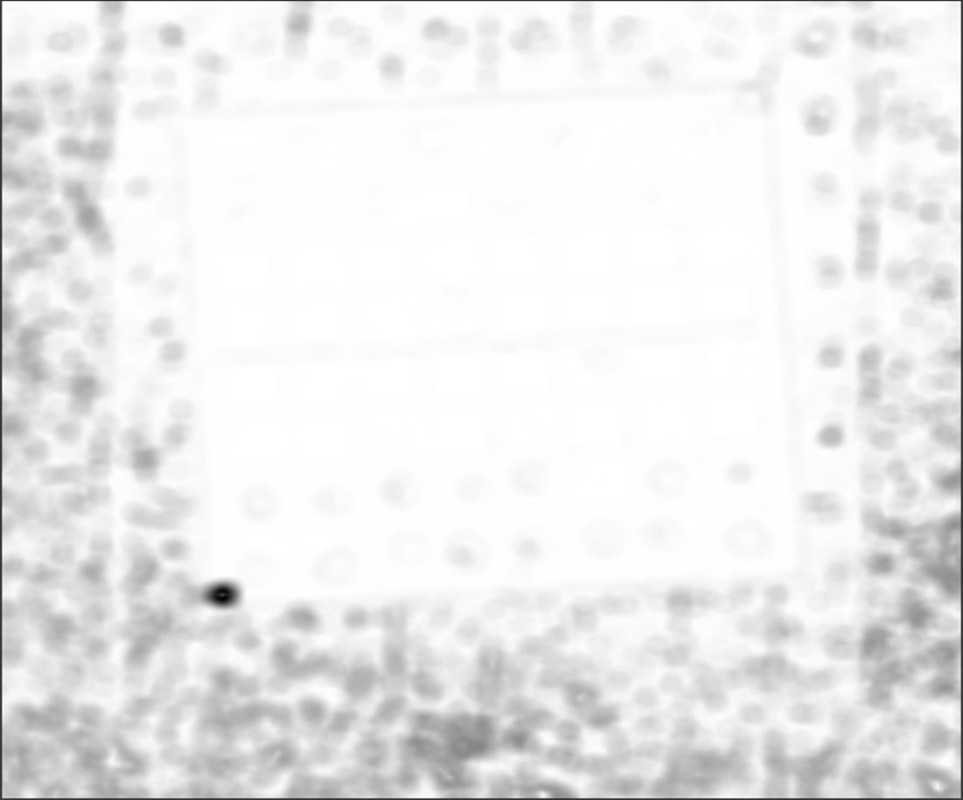
\includegraphics[width=\linewidth]{Pictures/Vision/Result.png}
        \caption{result of matchTemplate()}
        \label{fig:resultOfMatchTemplate()}
    \end{subfigure}
    \hfill
    \begin{subfigure}[t]{0.32\linewidth}
        \centering
        
\includegraphics[width=0.83\linewidth]{Pictures/Vision/circleMask.png}
        \caption{Mask and template image being used}
        \label{fig:mask}
    \end{subfigure}
    
    \caption{The image matchTemplate() is used on, the result and the mask and template image being used.}
    \label{fig:matchTemplateResult}
\end{figure}
The darkest spot of the result image corresponds to the location of the tape and can therefore be retrieved.

When the position of the corners have been located, the rotation can be found using atan, since the chessboard is a square. The same can be done for the pegs by placing them in a square. The angle can be calculated by \cref{eq:angleCal}
\begin{equation}
    \theta = atan\left(\frac{\Delta y}{\Delta x}\right) - \frac{\pi}{4}
    \label{eq:angleCal}
\end{equation}

Since $\theta$ is diagonal, the rotation needs to be offset by 45 \degrees clockwise.
By finding the pegs, calculating the angle, cutting the image and doing the same with the chessboard, a single image can be found of the chessboard, no matter the location or rotation, as long as its corners are inside the pegs' area. This can be seen in \cref{fig:Cut Boards}
The angle of the chessboard can also be used to define if the player wants to play as white or black just by turning the white or black of the chessboard to the player.
\begin{figure}[H]
    \centering
    \begin{subfigure}[t]{0.43\linewidth}
        \centering
        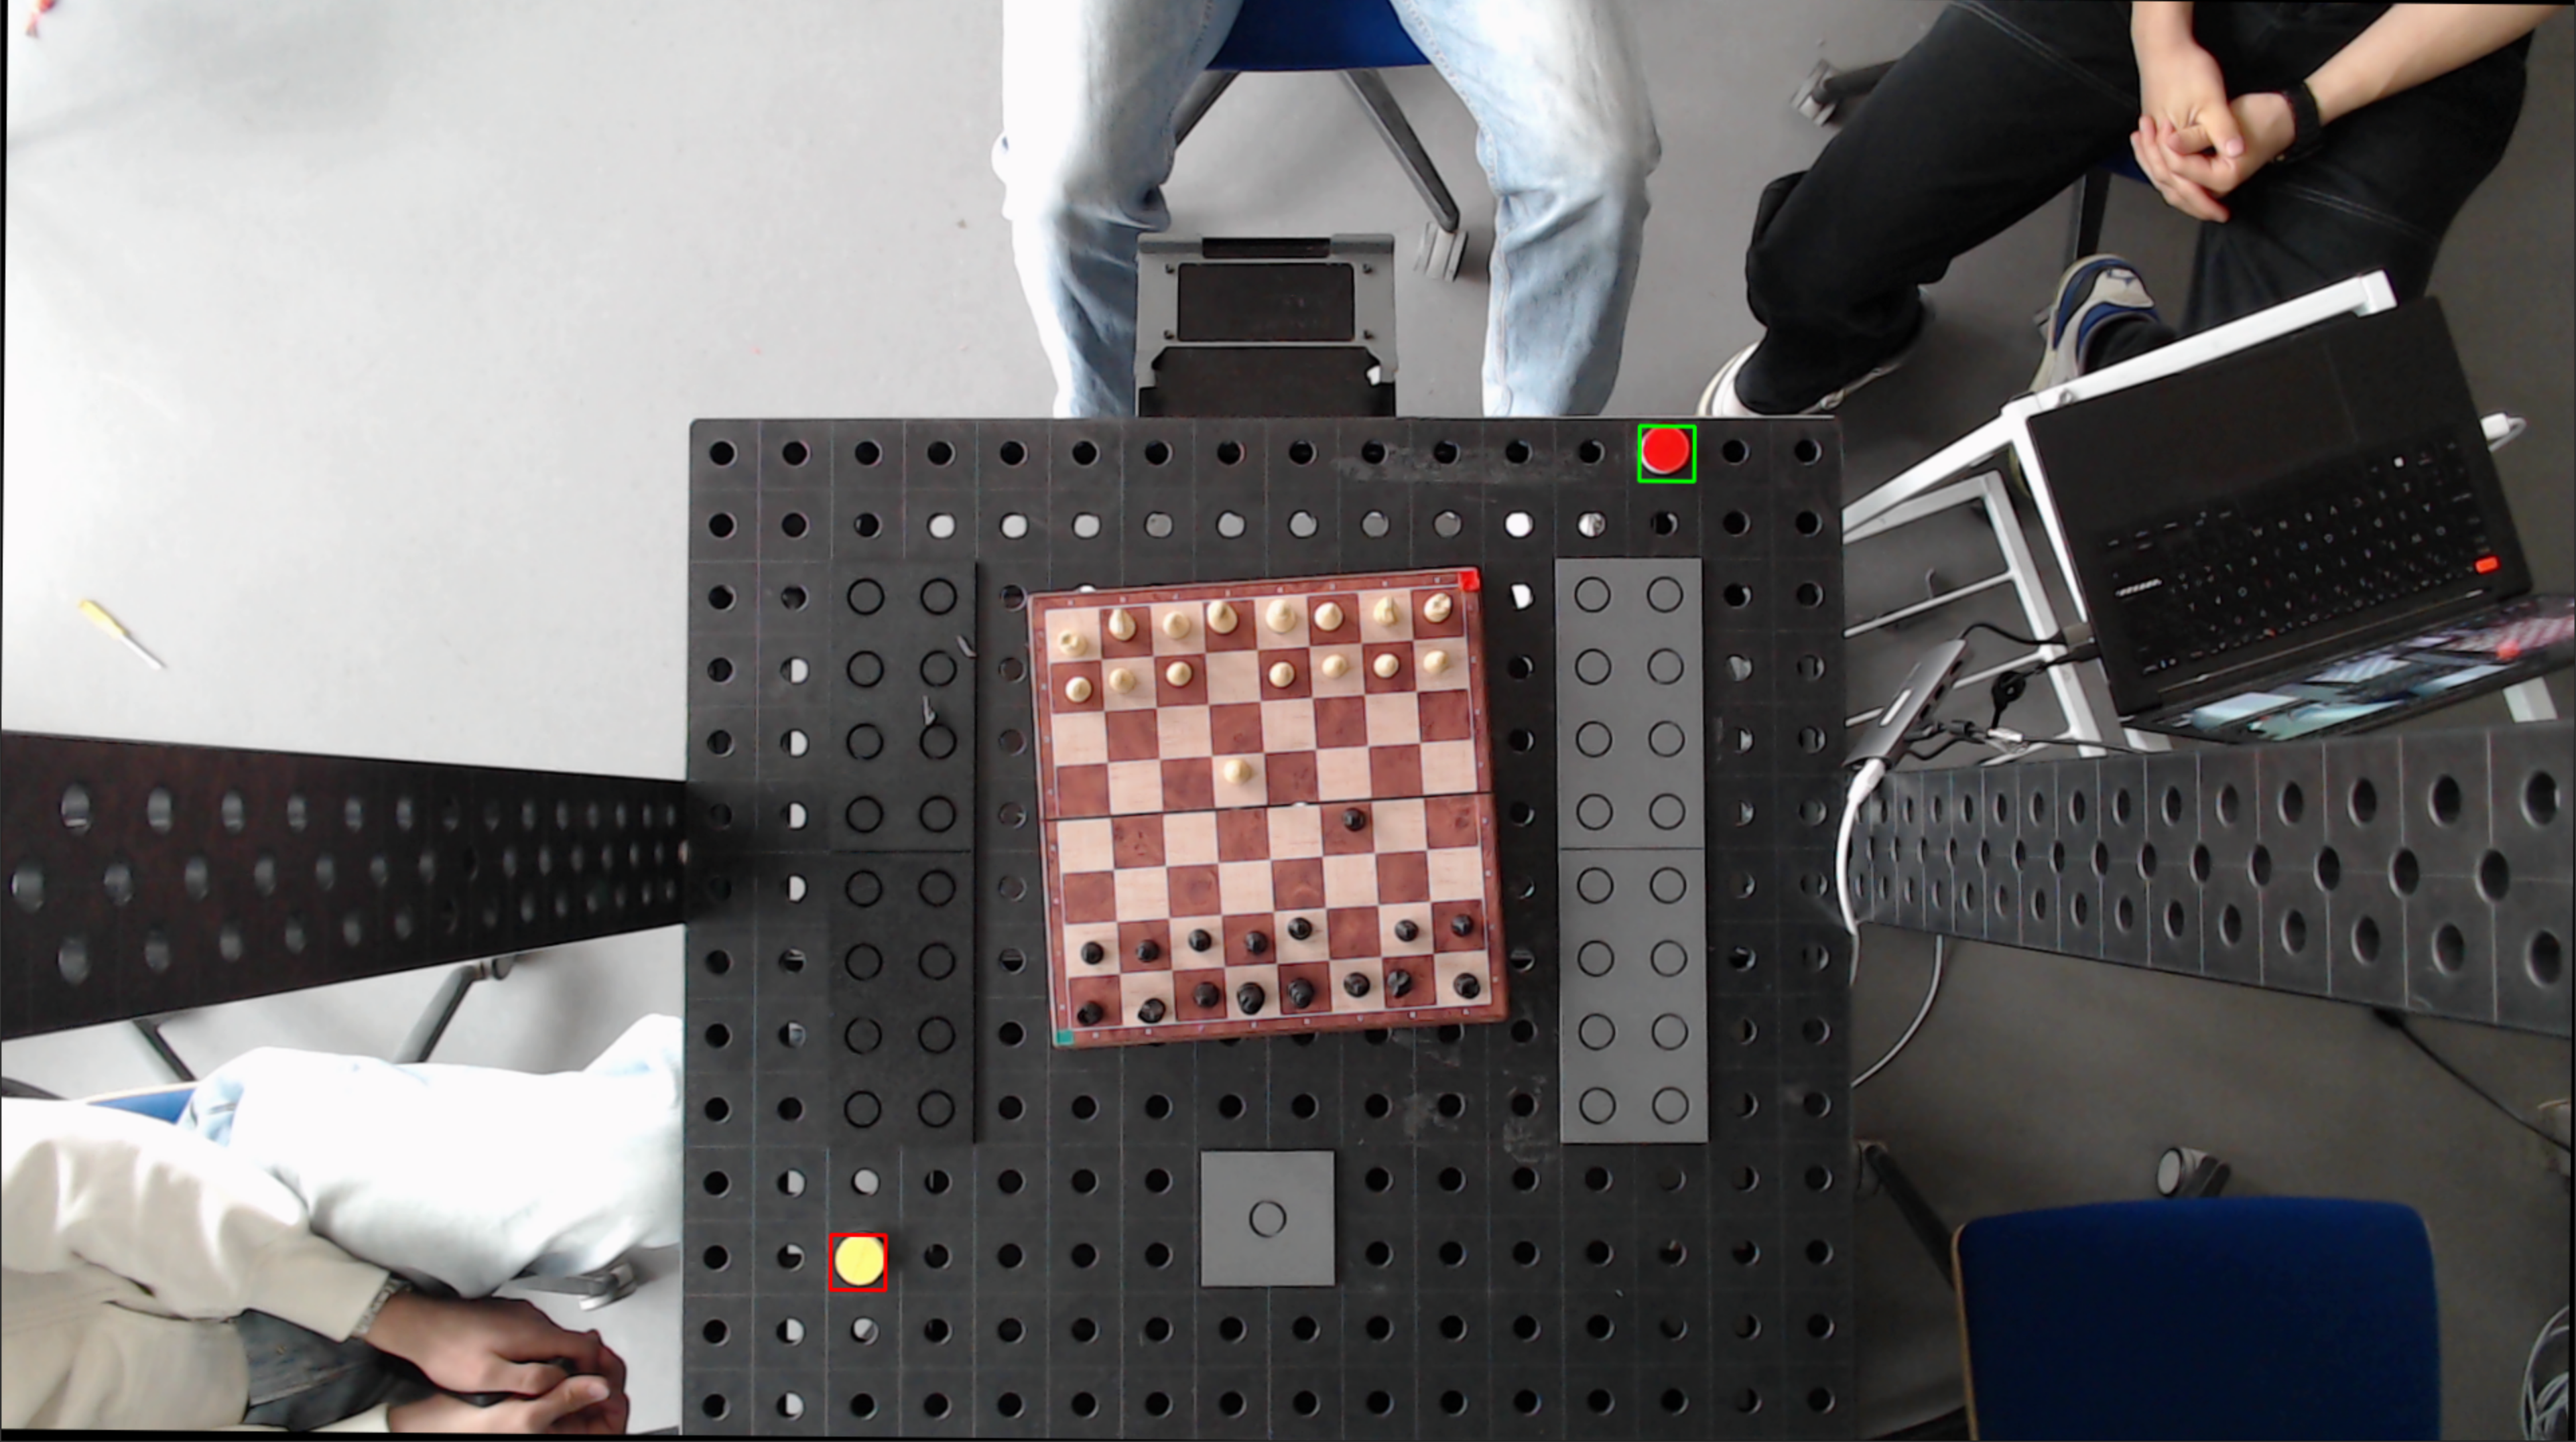
\includegraphics[width=\linewidth]{Pictures/Vision/PostRotationFirstCut.png}
        \caption{Original image with pegs marked}
        \label{fig:originalImageWithMarkedCorners}
    \end{subfigure}
    \hfill
    \begin{subfigure}[t]{0.24\linewidth}
        \centering
        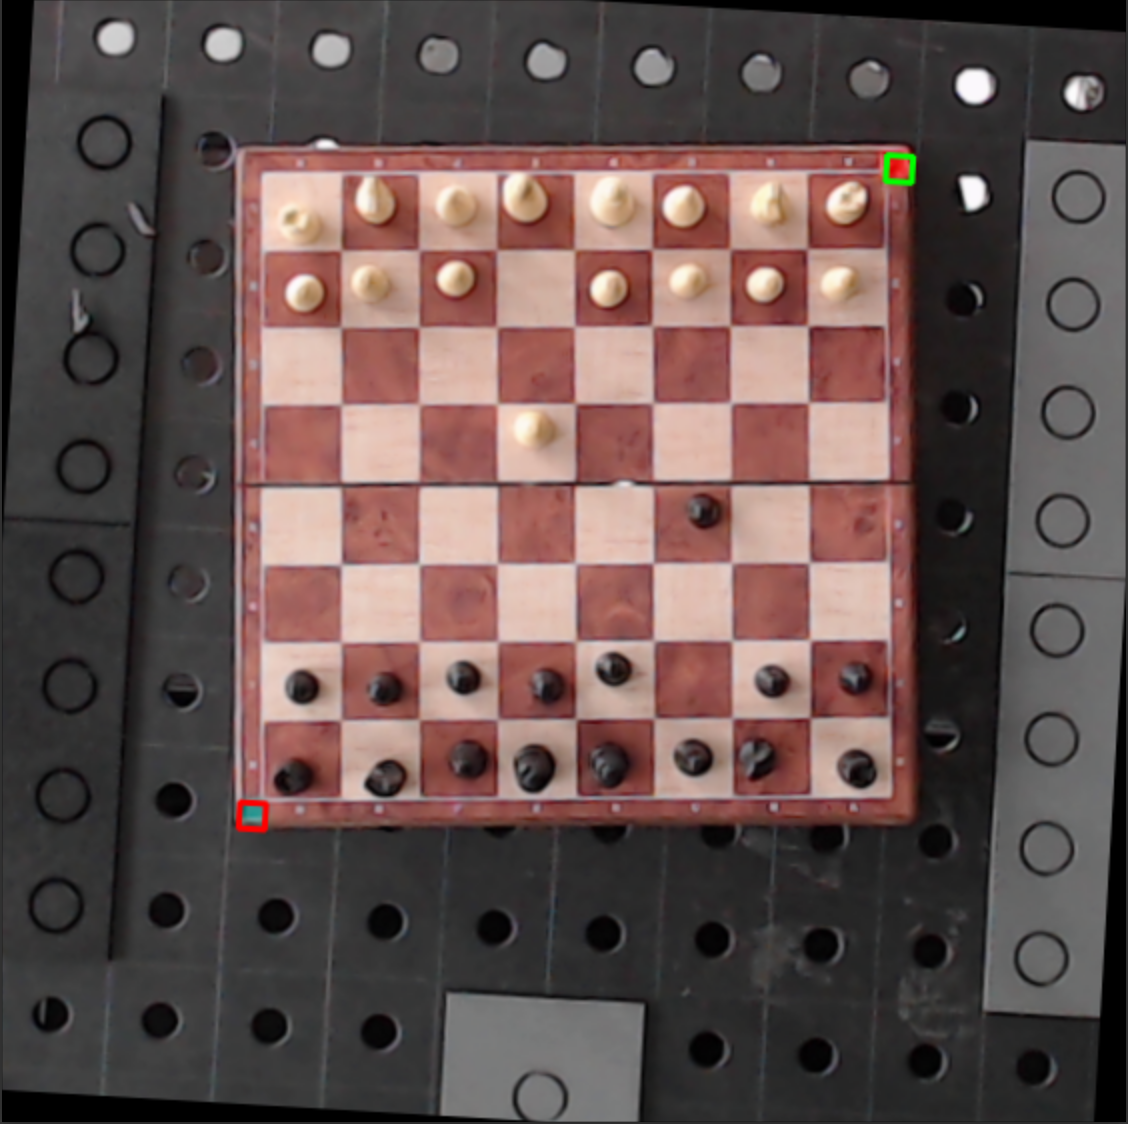
\includegraphics[width=\linewidth]{Pictures/Vision/PostRotationSecondCut.png}
        \caption{Cut image with the corners marked}
        \label{fig:firstcut}
    \end{subfigure}
    \hfill
    \begin{subfigure}[t]{0.24\linewidth}
        \centering
        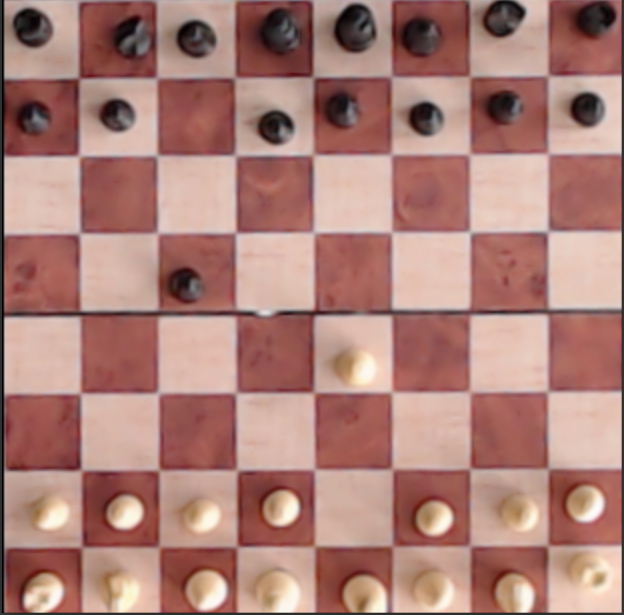
\includegraphics[width=\linewidth]{Pictures/Vision/FinalCut.png}
        \caption{Image cut down to the chessboard}
        \label{fig:finalCut}
    \end{subfigure}
    
    \caption{The original image with the pegs marked, the cut image with the chessboard corners marked and then the cut image again}
    \label{fig:Cut Boards}
\end{figure}

\subsection{Finding the player's move}
By comparing an image of the chessboard before and after the player has made a move, the difference tells us what piece the player has moved. As in \cref{sec: Locate tape} the channels can be processed separately and subtracted from each other. To make the difference more apparent compared to the rest of the image, the values in the channels can be raised to an exponent and normalized back again. This effect can be seen in \cref{fig:exponent}

\begin{figure}[H]
    \centering
    \begin{subfigure}[t]{0.49\linewidth}
        \centering
        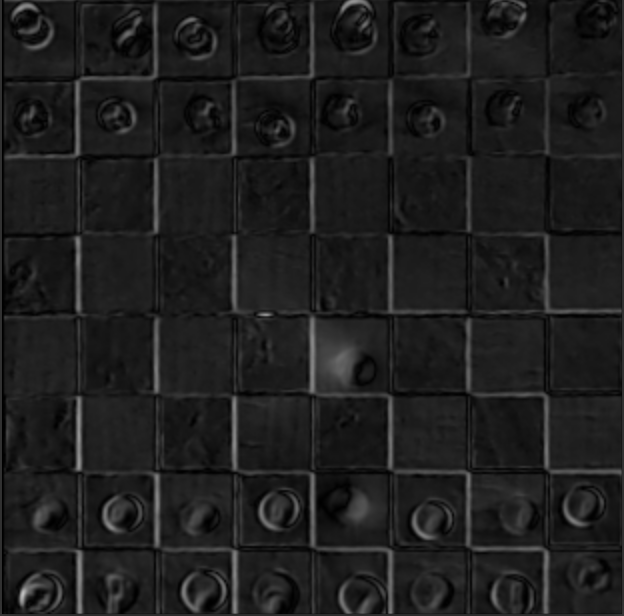
\includegraphics[width=0.8\linewidth]{Pictures/Vision/SaturationBeforeExponent.png}
        \caption{saturation channel before being squared} 
        \label{fig:valueBeforeExponent}
    \end{subfigure}
    \begin{subfigure}[t]{0.49\linewidth}
        \centering
        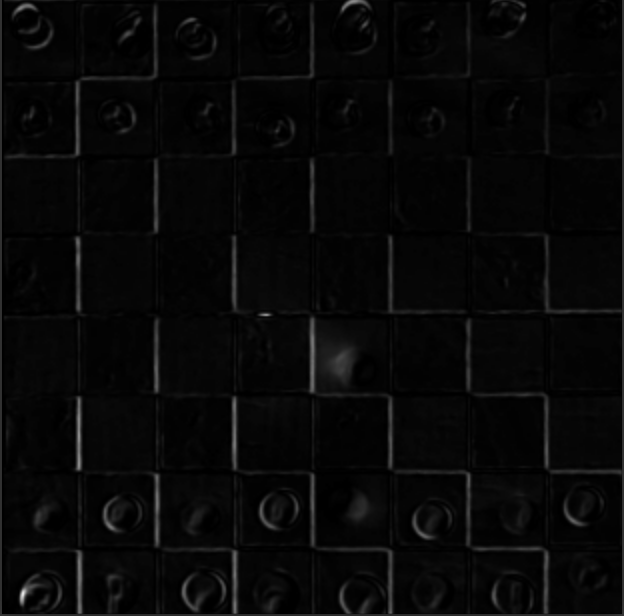
\includegraphics[width=0.8\linewidth]{Pictures/Vision/SaturationAfterExponent.png}
        \caption{saturation channel after being squared and normalized}
        \label{fig:valueAfterExponent}
    \end{subfigure}
    \caption{The saturation channel before and after being squared and normalized}
    \label{fig:exponent}
\end{figure}

Likewise when finding the corners of the chessboard, the weights for the channels has been found experimentally and are: Value and hue is 1 and saturation is 4.
Every channel is also squared to enhance the difference.

After squaring the values of all channels, the weighted average can be calculated.
This can be seen in \cref{fig:diffBoardWithLines}.

\begin{figure}[H]
    \centering
    \begin{subfigure}[t]{0.49\linewidth}
        \centering
        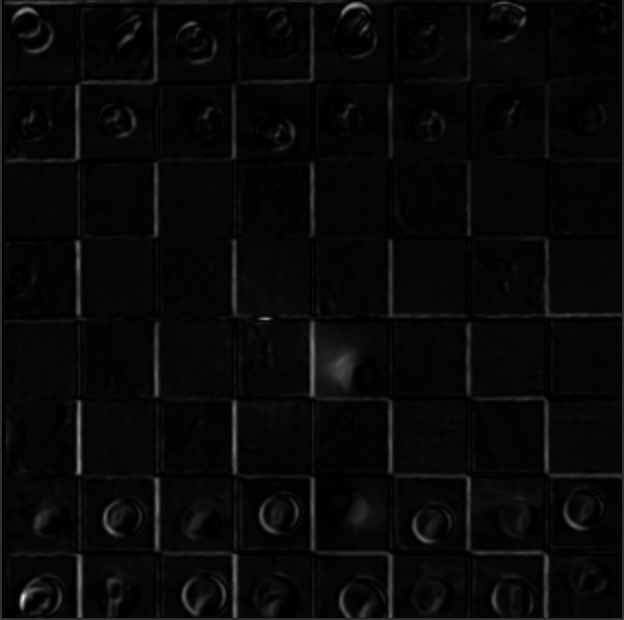
\includegraphics[width=0.8\linewidth]{Pictures/Vision/DiffBoard.png}
        \caption{Image with grid lines resulting from noise} 
        \label{fig:diffBoardWithLines}
    \end{subfigure}
    \begin{subfigure}[t]{0.49\linewidth}
        \centering
        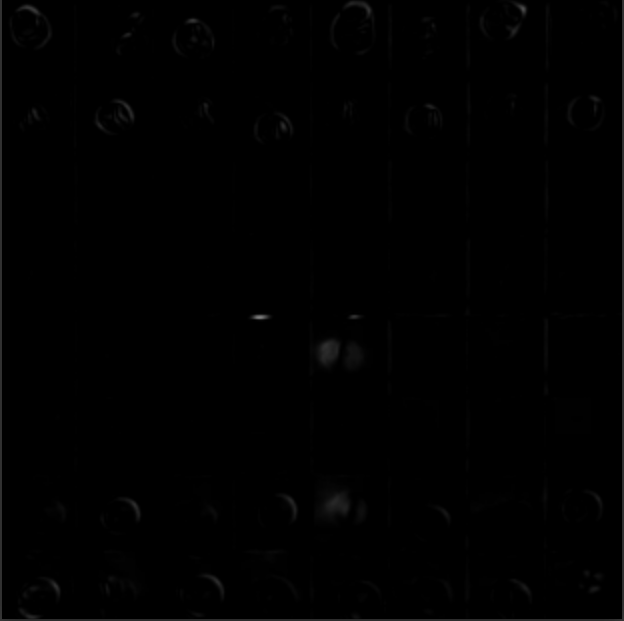
\includegraphics[width=0.8\linewidth]{Pictures/Vision/DiffBoardModified.png}
        \caption{Image with noise reduced resulting in no grid lines}
        \label{fig:diffBoardWithoutLines}
    \end{subfigure}
    \caption{Weighted average of the HSV channels before and after the player has made their move}
\end{figure}

When the camera finds the corners of the chessboard, it might have some noise, resulting in the location changing by a couple of pixels, every time. When a pixel with the position (x, y) is white on one image, it might be black in the next image, because of the noise. This can be seen in \cref{fig:diffBoardWithLines}.

This can be greatly mitigated by reducing the values for the pixels close to the border of each square. This effect can be seen in \cref{fig:diffBoardWithoutLines}.

Then for every tile on the chessboard the value for each pixel can be summed up to give that tile a score on how likely it is a piece has moved to or moved from it.
Then every tile value is summed with every other tile, and therefore creates $64^2$ tile pairs with a value which describes how likely it is for a piece to move from one of the tiles to the other. This can then be sorted to find the most likely move which the player has made.
However, accidentally touching a piece, and moving it slightly, can result in a significantly higher difference, making this tile added with any other tile, always have a higher score than the actual tiles for the move added together. This often occurs when touching a white piece on a black tile, and then moving a white piece, from a white tile to a new white tile. To solve this, a function to reduce the relative high values and increase the relative low values is being applied to the tile scores. The values are first normalized to be between 0 and 5, and then raised to $\frac{1}{3}$ which has the effect that can be seen in \cref{fig:graphs}.

\begin{figure} [H]
    \centering
    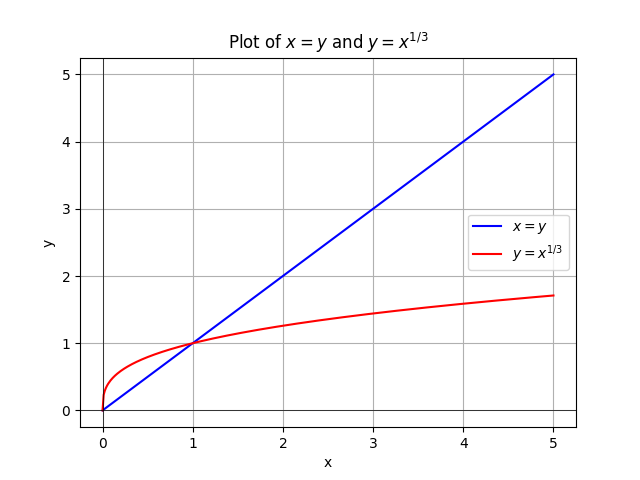
\includegraphics[width=0.6\linewidth]{Pictures/Vision/Figure_1.png}
    \caption{Image of the graph $y=x^\frac{1}{3}$ compared to $y=x$}
    \label{fig:graphs}
\end{figure}

This reduces the dominance of just 1 square having a high value.

When the player castles or performs en passant, the change in square values spans 4 and 3 squares respectively, which can't be evaluated like standard moves. To handle this, special scores are added to the list of possible moves.

For castling, the involved four squares are summed and divided by 1.5. Dividing by 2 would incorrectly treat it like a normal move, and dividing by 1 would overvalue it, causing the system to always assume a castle, even when the king and rook simply move closer. This happens because the changed squares from castling can skew the scoring.

A similar adjustment is made for en passant.

To further increase consistency, the most likely move is detected for legality. If it is an illegal move, the second most likely move is checked, and so on. This requires a way of validating moves. For this a move validator program is used.